\documentclass[handout]{beamer}\usepackage[]{graphicx}\usepackage[]{color}
%% maxwidth is the original width if it is less than linewidth
%% otherwise use linewidth (to make sure the graphics do not exceed the margin)
\makeatletter
\def\maxwidth{ %
  \ifdim\Gin@nat@width>\linewidth
    \linewidth
  \else
    \Gin@nat@width
  \fi
}
\makeatother

\definecolor{fgcolor}{rgb}{0, 0, 0}
\newcommand{\hlnum}[1]{\textcolor[rgb]{0.533,0,0.133}{#1}}%
\newcommand{\hlstr}[1]{\textcolor[rgb]{0.667,0.267,0}{#1}}%
\newcommand{\hlcom}[1]{\textcolor[rgb]{1,0.533,0}{#1}}%
\newcommand{\hlopt}[1]{\textcolor[rgb]{0,0,0}{\textbf{#1}}}%
\newcommand{\hlstd}[1]{\textcolor[rgb]{0,0,0}{#1}}%
\newcommand{\hlkwa}[1]{\textcolor[rgb]{0.4,0.067,0.067}{\textbf{#1}}}%
\newcommand{\hlkwb}[1]{\textcolor[rgb]{0,0,0.4}{\textbf{#1}}}%
\newcommand{\hlkwc}[1]{\textcolor[rgb]{0,0,0.4}{#1}}%
\newcommand{\hlkwd}[1]{\textcolor[rgb]{0,0.267,0.4}{#1}}%
\let\hlipl\hlkwb

\usepackage{framed}
\makeatletter
\newenvironment{kframe}{%
 \def\at@end@of@kframe{}%
 \ifinner\ifhmode%
  \def\at@end@of@kframe{\end{minipage}}%
  \begin{minipage}{\columnwidth}%
 \fi\fi%
 \def\FrameCommand##1{\hskip\@totalleftmargin \hskip-\fboxsep
 \colorbox{shadecolor}{##1}\hskip-\fboxsep
     % There is no \\@totalrightmargin, so:
     \hskip-\linewidth \hskip-\@totalleftmargin \hskip\columnwidth}%
 \MakeFramed {\advance\hsize-\width
   \@totalleftmargin\z@ \linewidth\hsize
   \@setminipage}}%
 {\par\unskip\endMakeFramed%
 \at@end@of@kframe}
\makeatother

\definecolor{shadecolor}{rgb}{.97, .97, .97}
\definecolor{messagecolor}{rgb}{0, 0, 0}
\definecolor{warningcolor}{rgb}{1, 0, 1}
\definecolor{errorcolor}{rgb}{1, 0, 0}
\newenvironment{knitrout}{}{} % an empty environment to be redefined in TeX

\usepackage{alltt}
%\usepackage{pgfpages}
%\pgfpagesuselayout{4 on 1}[a4paper,border shrink=5mm,landscape]
\newenvironment{changemargin}[2]{%
\begin{list}{}{%
\setlength{\topsep}{0pt}%
\setlength{\leftmargin}{#1}%
\setlength{\rightmargin}{#2}%
\setlength{\listparindent}{\parindent}%
\setlength{\itemindent}{\parindent}%
\setlength{\parsep}{\parskip}%
}%
\item[]}{\end{list}}
\usepackage{graphicx}
\usepackage{amsmath}
\usepackage{url}
\usetheme{Madrid}
\usecolortheme{beaver}
\setbeamertemplate{navigation symbols}{}
\titlegraphic{
\includegraphics[width=5cm]{..//..//S-DS-VC-RGB.png}}
%\logo{
\includegraphics[width=0.1\textwidth,keepaspectratio]{..//..//UOACrest.png}}
\author[SCC]{Statistical Consulting Centre}%\\
\institute[\href{mailto:consulting@stat.auckland.ac.nz}
  {consulting@stat.auckland.ac.nz}]{\href{mailto:consulting@stat.auckland.ac.nz}
  {consulting@stat.auckland.ac.nz}\\
%Statistical Consulting Centre\\
The Department of Statistics\\
The University of Auckland}
\title[Session 1 -- Introduction]{NZSSN Courses: Introduction to \texttt{R}}
\subtitle{Session 1 -- Introduction} 
%\subtitle{Stats 780}
\date{1 March, 2017}
\IfFileExists{upquote.sty}{\usepackage{upquote}}{}
\begin{document}
%\SweaveOpts{concordance=TRUE}


\maketitle

\begin{frame}
  \frametitle{Wednesday}

\begin{center}
Each session comprises two parts: lecture and practice.
\end{center}
  \begin{table}[h]
    \centering
    \begin{tabular}[h]{lll}
     \hline
     \textbf{Session} & \textbf{Time}     & \textbf{Session}  \\
     \hline
     1            & 09:00am - 10:30am & Introduction          \\
                  & 10:30am - 10:50am & Break             \\
     2            & 10:50am - 01:00pm & Subsetting data \\
                  & 01:00pm - 02:00pm & Lunch break        \\
     3            & 02:00pm - 03:00pm & Data manipulation        \\
                  & 03:00pm - 03:20pm & Break             \\
     4            & 03:20pm - 04:30pm & Data exploration         \\
     \hline
    \end{tabular}
  \end{table}
\end{frame}

\begin{frame}
  \frametitle{Thursday}

  \begin{table}[h]
    \centering
    \begin{tabular}[h]{lll}
     \hline
     \textbf{Session} & \textbf{Time}     & \textbf{Session}  \\
     \hline
     1          & 09:00am - 10:30am & Graphics          \\
                & 10:30am - 10:50am & Break             \\
     2          & 10:50am - 12:30pm & Advanced Graphics \\
                & 12:30pm - 01:30pm & Lunch break        \\
     3          & 01:30pm - 03:00pm & Simple analysis        \\
                & 03:00pm - 03:20pm & Break             \\
     4          & 03:20pm - 04:30pm & Advanced analysis     \\
     \hline
    \end{tabular}
  \end{table}
\end{frame}

\begin{frame}
  \frametitle{\texttt{R} and UoA's Department of Statistics}
  \begin{itemize}
  \item \texttt{R} was initially written by Robert Gentleman and Ross
    Ihaka -- \textit{R \& R} -- of the \textbf{\textcolor{blue}{Department of Statistics,
      University of Auckland}}.
  \item Three members of the \textit{R Development Core Team} are in
    UoA's Department of Statistics.
  \end{itemize}
  \centering
  
\includegraphics[width=5cm]{..//..//S-DS-VC-RGB.png}
\end{frame}


\begin{frame}
  \frametitle{\texttt{R} and UoA's Department of Statistics}
  \begin{figure}[h]
    \centering
    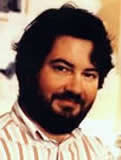
\includegraphics[width = .3\textwidth, keepaspectratio]{ross.jpg}
  \end{figure}
   \begin{center}
     \Large Ross Ihaka
   \end{center}
\end{frame}

\begin{frame}
  \frametitle{\texttt{R} and UoA's Department of Statistics}
  \begin{figure}[h]
    \centering
    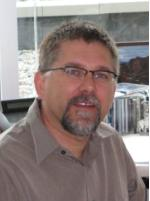
\includegraphics[width = .3\textwidth, keepaspectratio]{rob.jpg}
  \end{figure}
   \begin{center}
     \Large Robert Gentleman (no longer in our department)
   \end{center}
\end{frame}

\begin{frame}
  \frametitle{\texttt{R} and UoA's Department of Statistics}
  \begin{figure}[h]
    \centering
    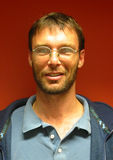
\includegraphics[width = .3\textwidth, keepaspectratio]{paul.jpg}
  \end{figure}
   \begin{center}
     \Large Paul Murrell
   \end{center}
\end{frame}


\begin{frame}
  \frametitle{\texttt{R} and UoA's Department of Statistics}
  \begin{figure}[h]
    \centering
    \includegraphics[width = .3\textwidth, keepaspectratio]{thomas.jpg}
  \end{figure}
   \begin{center}
     \Large Thomas Lumley
   \end{center}
\end{frame}

\begin{frame}
  \frametitle{\texttt{R} and UoA's Department of Statistics}
  \begin{block}{What does this mean?}
    \textit{If you want to learn \texttt{R}, you are talking to the right people!}
  \end{block}
  \begin{figure}[h]
    \centering
    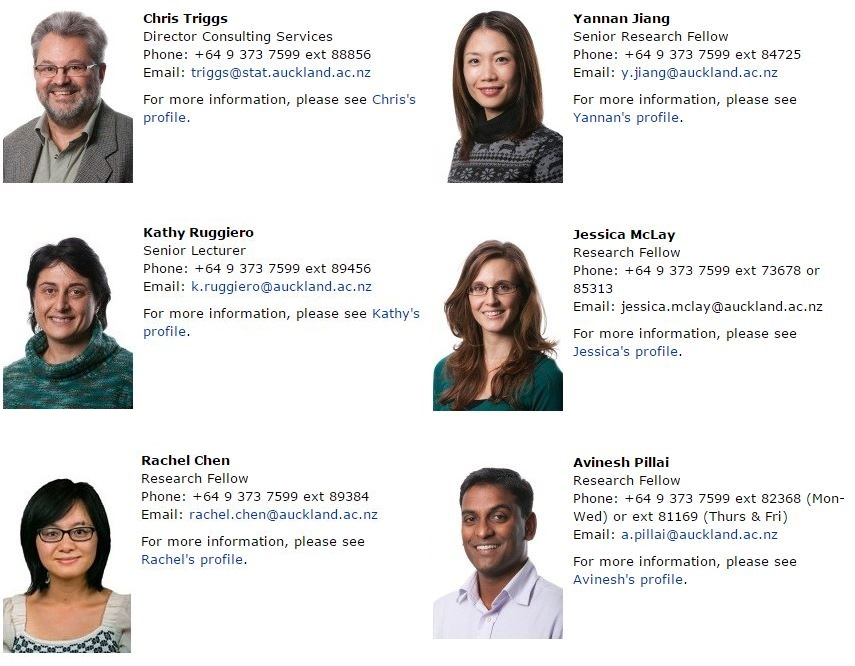
\includegraphics[width = .7\textwidth, keepaspectratio]{groupNew.jpg}
  \end{figure}
\end{frame}

\begin{frame}
  \begin{block}{What is \texttt{R}?}
    ``\texttt{R} is a free software environment for statistical computing and graphics''
  \end{block}
Key words:
  \begin{itemize}
    \item FREE!!!!!
    \item Statistical computing
    \item Graphics (much more flexible than SAS, SPSS, JMP, etc.)
    \item Support from communities of different fields, i.e. \texttt{R} packages. \url{https://cran.r-project.org/web/views/}.
    \item Even Microsoft is in it: Microsoft R Open. \url{https://mran.microsoft.com/open/}.
  \end{itemize}
\end{frame}


\begin{frame}
  \frametitle{The \texttt{R} Graphical User Interface (GUI)}
  \begin{figure}[h]
    \centering
    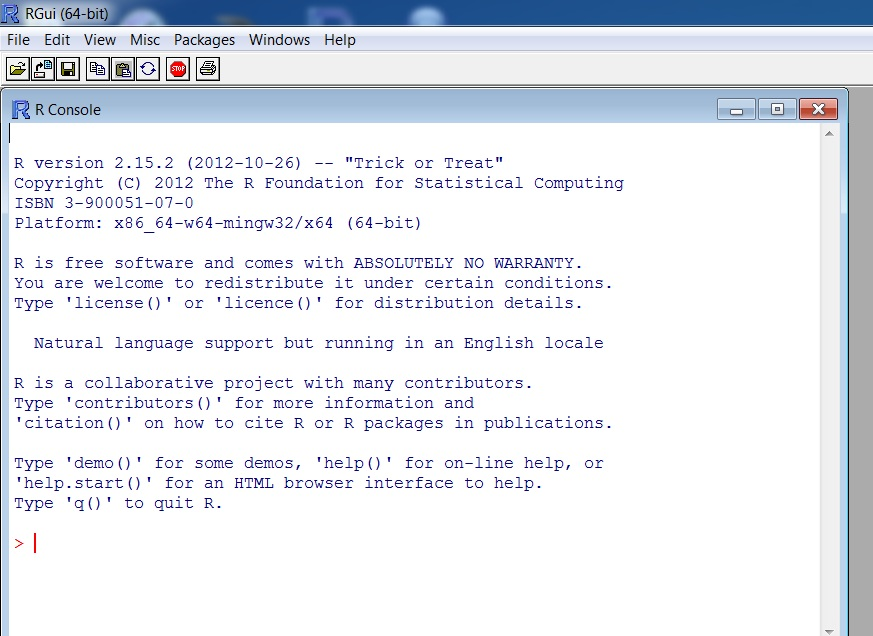
\includegraphics[width = 1\textwidth, keepaspectratio]{Rgui.jpg}
  \end{figure}
\end{frame}


\begin{frame}
  \frametitle{How to download and install \texttt{R}}
  \begin{enumerate}
  \item Go to the CRAN (Comprehensive R Archive Network)
    \url{cran.stat.auckland.ac.nz}.
  \item Download the relevant version for Linux/Mac/Windows.
    \begin{itemize}
    \item We will only look at \texttt{R} in the Windows environment today.
    \end{itemize}
  \item Install it on your computer (for Windows only):
    \begin{itemize}
    \item Choose ``Yes (customized startup)'' in Startup options.
    \item Choose ``SDI (separate windows)'' in Display mode.
    \item Choose ``HTML help'' in Help .
    \end{itemize}
  \end{enumerate}
\end{frame}


\begin{frame}
  \frametitle{Using the \texttt{R} editor}
  \begin{itemize}
    \item The \texttt{R} GUI is not menu driven.
    \item Commands can be typed at the console.
    \begin{itemize}
      \item OK for simple calculations requiring few lines of code
      \item Painful for anything more!
    \end{itemize}
    \item We \emph{strongly} recommend using an \texttt{R} editor
    \begin{itemize}
      \item Great for reproducible analyses and research!!
      \item Best editor for you depends on whether you are a(n)...
      \begin{enumerate}
        \item Beginner: Built-in \texttt{R} editor,
        \item Advanced user: \texttt{R}studio, Tinn-R, Notepad++, and many others.
        \item \texttt{R} geek: Emacs
      \end{enumerate}
    \end{itemize}
  \end{itemize}
\end{frame}
\begin{frame}[fragile]
  \frametitle{Using \texttt{R} as a calculator}
\begin{knitrout}
\definecolor{shadecolor}{rgb}{0.969, 0.969, 0.969}\color{fgcolor}\begin{kframe}
\begin{alltt}
\hlnum{1}\hlopt{+}\hlnum{2}
\end{alltt}
\begin{verbatim}
[1] 3
\end{verbatim}
\end{kframe}
\end{knitrout}
\begin{knitrout}
\definecolor{shadecolor}{rgb}{0.969, 0.969, 0.969}\color{fgcolor}\begin{kframe}
\begin{alltt}
\hlnum{1} \hlopt{+} \hlnum{3}\hlopt{^}\hlnum{2}
\end{alltt}
\begin{verbatim}
[1] 10
\end{verbatim}
\end{kframe}
\end{knitrout}
\begin{knitrout}
\definecolor{shadecolor}{rgb}{0.969, 0.969, 0.969}\color{fgcolor}\begin{kframe}
\begin{alltt}
\hlkwd{log}\hlstd{(}\hlnum{15}\hlstd{)} \hlopt{-} \hlkwd{sqrt}\hlstd{(}\hlnum{3.4}\hlstd{)}
\end{alltt}
\begin{verbatim}
[1] 0.8641413
\end{verbatim}
\end{kframe}
\end{knitrout}
\begin{knitrout}
\definecolor{shadecolor}{rgb}{0.969, 0.969, 0.969}\color{fgcolor}\begin{kframe}
\begin{alltt}
\hlkwd{pnorm}\hlstd{(}\hlnum{1.96}\hlstd{)}
\end{alltt}
\begin{verbatim}
[1] 0.9750021
\end{verbatim}
\end{kframe}
\end{knitrout}
\end{frame}


\begin{frame}[fragile]
  \frametitle{Using \texttt{R} as a calculator}
  \begin{itemize}
  \item "\verb|<-|" is the "assign to" operator, made up of "\verb|<|" and "\verb|-|" without a space.
  \item E.g., \verb|x <- 2| is read as "The value 2 is assigned to the object \verb|x|".
\begin{knitrout}
\definecolor{shadecolor}{rgb}{0.969, 0.969, 0.969}\color{fgcolor}\begin{kframe}
\begin{alltt}
\hlstd{x} \hlkwb{<-} \hlnum{2}
\hlstd{y} \hlkwb{<-} \hlnum{3}
\hlstd{x}\hlopt{^}\hlnum{2} \hlopt{-} \hlnum{3}\hlopt{*}\hlstd{y} \hlopt{+} \hlnum{5}
\end{alltt}
\begin{verbatim}
[1] 0
\end{verbatim}
\end{kframe}
\end{knitrout}
%\item \verb|<-| operates \emph{almost} the same as $=$, but \emph{not
 %   exactly} the same as $=$.
\item \verb|<-| has a direction, from right to left, \verb|x <- 2| means
  assigning 2 to $x$,
\end{itemize}
\end{frame}


\begin{frame}[fragile]
  \frametitle{Using \texttt{R} as a calculator}
  \begin{itemize}
\item \verb|->| operates from left to right, assigning $x$ to 2. \\
2 is a real value so you can not do that.
\begin{knitrout}
\definecolor{shadecolor}{rgb}{0.969, 0.969, 0.969}\color{fgcolor}\begin{kframe}
\begin{alltt}
\hlstd{x} \hlkwb{->} \hlnum{2}
\end{alltt}


{\ttfamily\noindent\bfseries\color{errorcolor}{Error in 2 <- x: invalid (do\_set) left-hand side to assignment}}\end{kframe}
\end{knitrout}
\item $=$ has no direction and can be confusing sometimes.
\item It is good programming practice to use \verb|<-|.
\end{itemize}
\end{frame}


\begin{frame}
  \frametitle{Getting help}
  \begin{itemize}
  \item Google!!!!\\
    e.g. How to calculate the mean in \texttt{R}? The
    search results
    tell you that the function \texttt{mean()} would be helpful.
  \item Quick-R: \url{http://www.statmethods.net/}
  \item R-bloggers: \url{https://www.r-bloggers.com/}
  \end{itemize}
\end{frame}

\begin{frame}
  \frametitle{Getting help}
  \begin{itemize}
  \item \texttt{?} \\
  e.g. \texttt{?mean} brings up the help file for this function. It will tell
    you (almost) everything you need to know to use \texttt{mean()}.
   \item \texttt{??} \\
   e.g. \texttt{??mean} searches for everything related to mean in your computer.
   \item \texttt{RSiteSearch(" ")}\\
    Searches everything on CRAN as well as your computer.
  \end{itemize}
\end{frame}


\begin{frame}[fragile]
  \frametitle{Data, files, statisticians and \texttt{R}}
  \begin{itemize}
    \item Statisticians prefer (read: \textbf{\emph{want}}) rectangular data files
    \begin{itemize}
      \item Each case in its own row
      \item Data collected on each variable in its own column
      \item Variable names in the first row of each column
      \item No blanks, e.g. fill with NA, *, 99999, anything but a blank!
    \end{itemize}
    \item \texttt{R} likes (read: \textbf{\emph{needs}}) this too!
    \item \texttt{R} prefers to read data files in Comma Separated Value (CSV) format.
    \item This does not mean \texttt{R} only reads files stored in csv format.
  \end{itemize}
\end{frame}


\begin{frame}[fragile]
  \frametitle{Getting data into \texttt{R}}
  Try your best to save your data in a \texttt{csv} or
    \texttt{txt} format.
    \begin{itemize}
    \item Most datasets are saved in an Excel spreadsheet.
    \item Do as much data cleaning as you can in Excel. No comments,
      no formatting, no colours, no fancy fonts.
    \item Convert it into \texttt{csv} by clicking on \texttt{Save
        As}. Change the \texttt{Save
        as type} from \texttt{xlsx} or \texttt{xls} into \texttt{CSV
        (Comma Delimited)}.
    \item \texttt{CSV} can have one worksheet only. If you have
      multiple worksheets, it saves the active worksheet.
    \end{itemize}
\end{frame}

\begin{frame}
  \frametitle{\texttt{issp.df}}
  \begin{itemize}
\item International Social Survey Programme (ISSP): 1994 - Family and Changing Gender Roles II (Modified)
\item Question 1 to 4, choose from one of the following: Agree strongly, Agree, Neither agree nor disagree, Disagree, Disagree strongly, Can't choose.
  \end{itemize}
\begin{enumerate}
\item Both the man and the woman should contribute to the household income.
\item A man's job is to earn money: a woman's job is to look after the home and family.
\item It is not good if the man stays at home and cares for the children and the woman goes out to work.
\item Family life often suffers because men concentrate too much on their work.
\end{enumerate}
\end{frame}

\begin{frame}
\frametitle{\texttt{issp.df}}
\begin{enumerate}
\setcounter{enumi}{4}
\item Which of these would you say is more important in preparing children for life?\\
to be obedient, to think for themselves, or Can't choose.
\end{enumerate}
\begin{itemize}
\item Question 6 to 8, choose one of the following: \\
Always wrong, Almost always wrong, Wrong only sometimes, Not wrong at all, Can't choose.
\end{itemize}
\begin{enumerate}
\setcounter{enumi}{5}
\item Do you think it is wrong or not wrong if a man and a woman have sexual relations before marriage?
\item What if they are in their early teens, say under 16 years old, in that case is it...
\item What about a married person having sexual relations with someone other than his or her husband or wife, it is...
\end{enumerate}
\end{frame}

\begin{frame}
\frametitle{Eight additional variables in \texttt{issp.df}}
\begin{itemize}
\item ID: Identification number.
\item Gender.
\item Age.
\item Marital Status.
\item Education: Education level.
\item Working hours per week: the average number of hours per week.
\item Income: Individual annual income.
\item Ethnicity
\end{itemize}
\end{frame}


\begin{frame}[fragile]
\frametitle{Read and Check}
  \begin{itemize}
  \item Always set a working directory using \texttt{setwd()}, this can be a directory where you store the data and/or outputing the results.  
  \item Use \texttt{read.csv} to read a CSV file into \texttt{R}.
  \item \texttt{dim()}: Returns the number of observations (rows) and variables (columns).
  \item \texttt{head()}/\texttt{tail()}: Returns the first/last few rows of a data set.
  \item \texttt{str()}: Returns the structure of the dataset, e.g., dimension, column names, type of data object, first few values of each variable.
  \item \texttt{names()}: Returns the names of the variables contained in a dataset.
  \end{itemize}
\end{frame}


\begin{frame}[fragile]
\frametitle{Reading data into \texttt{R}}
\begin{knitrout}
\definecolor{shadecolor}{rgb}{0.969, 0.969, 0.969}\color{fgcolor}\begin{kframe}
\begin{alltt}
\hlkwd{setwd}\hlstd{(}\hlstr{"your working directory"}\hlstd{)}
\hlstd{issp.df} \hlkwb{<-} \hlkwd{read.csv}\hlstd{(}\hlstr{"issp.csv"}\hlstd{,} \hlkwc{stringsAsFactors} \hlstd{=} \hlnum{FALSE}\hlstd{)}
\hlkwd{head}\hlstd{(issp.df)}
\end{alltt}
\end{kframe}
\end{knitrout}
\begin{knitrout}
\definecolor{shadecolor}{rgb}{0.969, 0.969, 0.969}\color{fgcolor}\begin{kframe}
\begin{verbatim}
       ID                Q1                    Q2
1 1900073          disagree                 agree
2 1900013 strongly disagree neither agree nor dis
3 1900025          disagree     strongly disagree
4 1900037   cant choose, dk              disagree
5 1900043          disagree neither agree nor dis
6 1900061          disagree              disagree
\end{verbatim}
\end{kframe}
\end{knitrout}
\texttt{stringsAsFactors} argument is set to \texttt{FALSE}, so \textbf{character} vectors are not converted to \textbf{factor}s. We will cover the factor at Session 3. 
\end{frame}


\begin{frame}[fragile]
\frametitle{\texttt{dim()} and \texttt{str()}}
\begin{knitrout}
\definecolor{shadecolor}{rgb}{0.965, 0.965, 0.965}\color{fgcolor}\begin{kframe}
\begin{alltt}
\hlkwd{dim}\hlstd{(issp.df)}
\hlkwd{str}\hlstd{(issp.df)}
\end{alltt}
\end{kframe}
\end{knitrout}
\begin{knitrout}\small
\definecolor{shadecolor}{rgb}{0.965, 0.965, 0.965}\color{fgcolor}\begin{kframe}
\begin{verbatim}
[1] 1047   16
'data.frame':	1047 obs. of  10 variables:
 $ ID    : int  1900073 1900013 1900025 1900037 1900043 1900061 1900079 1900085 1900097 1900115 ...
 $ Q1    : chr  "disagree" "strongly disagree" "disagree" "cant choose, dk" ...
 $ Q2    : chr  "agree" "neither agree nor dis" "strongly disagree" "disagree" ...
 $ Q3    : chr  "neither agree nor dis" "disagree" "strongly disagree" "disagree" ...
 $ Q4    : chr  "agree" "agree" "agree" "agree" ...
 $ Q5    : chr  "think themselves" "think themselves" "think themselves" "can t choose, dk" ...
 $ Q6    : chr  "always wrong" "always wrong" "not wrong at all" "not wrong at all" ...
 $ Q7    : chr  "always wrong" "always wrong" "almost always wrong" "cant choose, dk" ...
 $ Q8    : chr  "always wrong" "always wrong" "only sometimes wrong" "always wrong" ...
 $ Gender: chr  "Female" "Male" "Female" "Female" ...
\end{verbatim}
\end{kframe}
\end{knitrout}
\end{frame}


\begin{frame}[fragile]
\frametitle{\texttt{names(issp.df)}}
\begin{knitrout}
\definecolor{shadecolor}{rgb}{0.965, 0.965, 0.965}\color{fgcolor}\begin{kframe}
\begin{alltt}
\hlcom{#Names of the variables}
\hlkwd{names}\hlstd{(issp.df)}
\end{alltt}
\begin{verbatim}
 [1] "ID"                     "Q1"                    
 [3] "Q2"                     "Q3"                    
 [5] "Q4"                     "Q5"                    
 [7] "Q6"                     "Q7"                    
 [9] "Q8"                     "Gender"                
[11] "Age"                    "Marital.Status"        
[13] "Education"              "Working.hours.per.week"
[15] "Income"                 "Ethnicity"             
\end{verbatim}
\end{kframe}
\end{knitrout}
\begin{itemize}
\item Anything following the \texttt{\#} symbol is treated as a comment and ignored by \texttt{R}.
\item Writing comments is a very good habit to develop!
\end{itemize}
\end{frame}

\begin{frame}[fragile]
  \frametitle{Descriptive statistics}
Calculate the mean of \texttt{Age}:
%\begin{verbatim}
%> mean(Age)
%Error in mean(Age) : object 'Age' not
%found
%\end{verbatim}
\begin{knitrout}
\definecolor{shadecolor}{rgb}{0.965, 0.965, 0.965}\color{fgcolor}\begin{kframe}
\begin{alltt}
\hlkwd{mean}\hlstd{(Age)}
\end{alltt}


{\ttfamily\noindent\bfseries\color{errorcolor}{Error in mean(Age): object 'Age' not found}}\end{kframe}
\end{knitrout}

You must tell \texttt{R} that \texttt{Age} is a variable (column)
\emph{within} \texttt{issp.df}, i.e.
\begin{knitrout}
\definecolor{shadecolor}{rgb}{0.965, 0.965, 0.965}\color{fgcolor}\begin{kframe}
\begin{alltt}
\hlkwd{mean}\hlstd{(issp.df}\hlopt{$}\hlstd{Age)}
\end{alltt}
\begin{verbatim}
[1] NA
\end{verbatim}
\end{kframe}
\end{knitrout}
You must also tell \texttt{R} how to deal with missing values: remove them before calculating the mean, i.e.
\begin{knitrout}
\definecolor{shadecolor}{rgb}{0.965, 0.965, 0.965}\color{fgcolor}\begin{kframe}
\begin{alltt}
\hlkwd{mean}\hlstd{(issp.df}\hlopt{$}\hlstd{Age,} \hlkwc{na.rm} \hlstd{=} \hlnum{TRUE}\hlstd{)}
\end{alltt}
\begin{verbatim}
[1] 45.77179
\end{verbatim}
\end{kframe}
\end{knitrout}
\end{frame}

\begin{frame}[fragile]
  \frametitle{\texttt{table} of counts}
\begin{knitrout}
\definecolor{shadecolor}{rgb}{0.965, 0.965, 0.965}\color{fgcolor}\begin{kframe}
\begin{alltt}
\hlcom{# One-way table of counts}

\hlkwd{table}\hlstd{(issp.df}\hlopt{$}\hlstd{Gender)}
\end{alltt}
\begin{verbatim}

     Female        Male NA, refused 
        607         418          22 
\end{verbatim}
\end{kframe}
\end{knitrout}
\end{frame}

\begin{frame}[fragile]
  \frametitle{\texttt{table} of proportions}
\begin{knitrout}
\definecolor{shadecolor}{rgb}{0.965, 0.965, 0.965}\color{fgcolor}\begin{kframe}
\begin{alltt}
\hlcom{# Total count}
\hlstd{total} \hlkwb{<-} \hlkwd{sum}\hlstd{(}\hlkwd{table}\hlstd{(issp.df}\hlopt{$}\hlstd{Gender))}
\hlstd{total}
\end{alltt}
\begin{verbatim}
[1] 1047
\end{verbatim}
\begin{alltt}
\hlcom{# Proportions of total}
\hlkwd{table}\hlstd{(issp.df}\hlopt{$}\hlstd{Gender)}\hlopt{/}\hlstd{total}
\end{alltt}
\begin{verbatim}

     Female        Male NA, refused 
 0.57975167  0.39923591  0.02101242 
\end{verbatim}
\end{kframe}
\end{knitrout}
\end{frame}

\begin{frame}[fragile]
  \frametitle{One-way tables \texttt{with} less typing}
Tired of typing \texttt{issp.df\$} over and over again? Use the \texttt{with} function.
\begin{knitrout}
\definecolor{shadecolor}{rgb}{0.965, 0.965, 0.965}\color{fgcolor}\begin{kframe}
\begin{alltt}
\hlstd{gender.table} \hlkwb{<-} \hlkwd{with}\hlstd{(issp.df,} \hlkwd{table}\hlstd{(Gender))}
\hlstd{gender.table}
\end{alltt}
\begin{verbatim}
Gender
     Female        Male NA, refused 
        607         418          22 
\end{verbatim}
\begin{alltt}
\hlstd{total} \hlkwb{<-} \hlkwd{sum}\hlstd{(gender.table)}
\hlstd{gender.table}\hlopt{/}\hlstd{total}
\end{alltt}
\begin{verbatim}
Gender
     Female        Male NA, refused 
 0.57975167  0.39923591  0.02101242 
\end{verbatim}
\end{kframe}
\end{knitrout}
\end{frame}

\begin{frame}[fragile]
  \frametitle{One-way tables \texttt{with} less typing}

\begin{knitrout}
\definecolor{shadecolor}{rgb}{0.965, 0.965, 0.965}\color{fgcolor}\begin{kframe}
\begin{alltt}
\hlcom{#Convert to percentages}
\hlstd{gender.pct} \hlkwb{<-} \hlnum{100}\hlopt{*}\hlstd{gender.table}\hlopt{/}\hlstd{total}
\hlstd{gender.pct}
\end{alltt}
\begin{verbatim}
Gender
     Female        Male NA, refused 
  57.975167   39.923591    2.101242 
\end{verbatim}
\begin{alltt}
\hlcom{# Round to 1 decimal place}
\hlkwd{round}\hlstd{(gender.pct,} \hlnum{1}\hlstd{)}
\end{alltt}
\begin{verbatim}
Gender
     Female        Male NA, refused 
       58.0        39.9         2.1 
\end{verbatim}
\end{kframe}
\end{knitrout}
\end{frame}

\begin{frame}[fragile]
  \frametitle{Two-way frequency tables}
\begin{knitrout}
\definecolor{shadecolor}{rgb}{0.965, 0.965, 0.965}\color{fgcolor}\begin{kframe}
\begin{alltt}
\hlstd{income.gender.tab} \hlkwb{<-} \hlkwd{with}\hlstd{(issp.df,} \hlkwd{table}\hlstd{(Income, Gender))}
\hlstd{income.gender.tab}
\end{alltt}
\begin{verbatim}
                        Gender
Income                   Female Male NA, refused
  $10000 or less            177   57           4
  $10001-$15000             115   35           2
  $15001-$20000              49   29           2
  $20001-$25000              65   50           0
  $25001-$30000              71   48           2
  $30001-$40000              59   70           4
  $40001-$50000              27   47           2
  $50001-$70000               7   27           1
  $70001-$100000              4   35           2
  NAV; NAP No own income     33   20           3
\end{verbatim}
\end{kframe}
\end{knitrout}
\end{frame}

\begin{frame}[fragile]
  \frametitle{Two-way frequency tables}
\begin{knitrout}\small
\definecolor{shadecolor}{rgb}{0.965, 0.965, 0.965}\color{fgcolor}\begin{kframe}
\begin{alltt}
\hlcom{# Calculate proportion with respect to 'margin' total}
\hlcom{# margin = 1 (row total) or 2 (column total) }
\hlstd{perc.income.gender} \hlkwb{<-} \hlkwd{prop.table}\hlstd{(income.gender.tab,} \hlkwc{margin}\hlstd{=}\hlnum{2}\hlstd{)}
\hlstd{perc.income.gender}
\end{alltt}
\begin{verbatim}
                        Gender
Income                        Female        Male
  $10000 or less         0.291598023 0.136363636
  $10001-$15000          0.189456343 0.083732057
  $15001-$20000          0.080724876 0.069377990
  $20001-$25000          0.107084020 0.119617225
  $25001-$30000          0.116968699 0.114832536
  $30001-$40000          0.097199341 0.167464115
  $40001-$50000          0.044481054 0.112440191
  $50001-$70000          0.011532125 0.064593301
  $70001-$100000         0.006589786 0.083732057
  NAV; NAP No own income 0.054365733 0.047846890
                        Gender
Income                   NA, refused
  $10000 or less         0.181818182
  $10001-$15000          0.090909091
  $15001-$20000          0.090909091
  $20001-$25000          0.000000000
  $25001-$30000          0.090909091
  $30001-$40000          0.181818182
  $40001-$50000          0.090909091
  $50001-$70000          0.045454545
  $70001-$100000         0.090909091
  NAV; NAP No own income 0.136363636
\end{verbatim}
\end{kframe}
\end{knitrout}
\end{frame}
\begin{frame}[fragile]
  \frametitle{Two-way frequency tables}
\begin{knitrout}
\definecolor{shadecolor}{rgb}{0.965, 0.965, 0.965}\color{fgcolor}\begin{kframe}
\begin{alltt}
\hlcom{# Tabulate as percentages}
\hlkwd{round}\hlstd{(}\hlnum{100}\hlopt{*}\hlstd{perc.income.gender,} \hlnum{1}\hlstd{)}
\end{alltt}
\begin{verbatim}
                        Gender
Income                   Female Male NA, refused
  $10000 or less           29.2 13.6        18.2
  $10001-$15000            18.9  8.4         9.1
  $15001-$20000             8.1  6.9         9.1
  $20001-$25000            10.7 12.0         0.0
  $25001-$30000            11.7 11.5         9.1
  $30001-$40000             9.7 16.7        18.2
  $40001-$50000             4.4 11.2         9.1
  $50001-$70000             1.2  6.5         4.5
  $70001-$100000            0.7  8.4         9.1
  NAV; NAP No own income    5.4  4.8        13.6
\end{verbatim}
\end{kframe}
\end{knitrout}
\end{frame}

\begin{frame}[fragile]
  \frametitle{Summary}
  \begin{itemize}
  \item Quick introduction to \texttt{R}
  \item Getting data into \texttt{R}
  \item Frequency tables
  \end{itemize}
\end{frame}

\end{document}
